\documentclass[11pt]{article}
\usepackage{fullpage}
\usepackage{hyperref}
\usepackage{listings}
\usepackage{graphicx}
\graphicspath{ {figs/} }

%\usepackage{doublespace}
\begin{document}
\title{Weekly Report - A rough Profiling Attempt to Ethash}
\author{MSc Project \\
Runchao Han \\
}
\maketitle
%
% This section is used to list the key action items from the
% previous meeting. This information will help provide 
% continuity of information and decisions made in the
% previous meeting. 
% Use the \item construct to list each item.  Try to keep the
% descriptions for each down to one or two sentences
%

%TODO references
\section{Progress of the Last Week}

\begin{enumerate}
\item Did a rough profiling to Ethash by adding timestamps
\item Learned about Nvidia GPU and CUDA programming
\item Learned about profiling CUDA programs by \texttt{nvprof} and \texttt{Nvidia Visual Profiler}
\end{enumerate}

\section{Introduction to CUDA profilers}

To profile CUDA programs, tools are involved. After searching for approaches, I found the only two profiling tools for CUDA programs:

\begin{itemize}
\item \texttt{nvprof}\footnote{http://docs.nvidia.com/cuda/profiler-users-guide/index.html}. This is a command line tool.
\item \texttt{Nvidia Visual Profiler}\footnote{http://www.sie.es/wp-content/uploads/2015/12/cuda-profiling-tools.pdf}. This is an Eclipse-based profiling tool which wraps \texttt{nvprof}.
\end{itemize}

A rough profiling was done by \texttt{nvprof}, by which a statistic was outputed, shown in Fig.~\ref{fig:nvprof_run_ethash_search}.


\begin{figure}[h]
    \centering
    \includegraphics[width=0.8\textwidth]{nvprof_run_ethash_search.eps}
    \caption{The \texttt{nvprof} result of $run\_ethash\_search()$.}
    \label{fig:nvprof_run_ethash_search}
\end{figure}

The result shows that $ethash\_calculate\_dag\_item()$ costs most of the time, which generates the whole 1GB DAG by a seed. However, the DAG generation can be pre-computed or copied from others, which makes optimising this process meaningless. The optimisation target is the mining process, which is the $compute\_hash()$ function in the code.

Currently, I have not succeeded in importing the project into \texttt{Nvidia Visual Profiler}. This is the main target next week.

\section{Profiling $compute\_hash()$ Function}

Due to the limitation of the command line, it is hard to get statistics of different steps which are set by myself. Therefore, I set timestamps manually in the code.

The steps of conducting the profiling are listed below:

\begin{enumerate}
	\item Set the CUDA mining function involves only one block and the block contains only one thread. 
		\begin{itemize}
		\item A CUDA Kernel function takes a grid (fixed)
		\item A grid takes several blocks (modifiable)
		\item A block takes several threads (modifiable)
		\end{itemize}
	\item Add timestamps in the code. The code involves steps listed below:
		\begin{enumerate}
		\item State initialisation
		\item An iteration of 4 (t)
			\begin{enumerate}
			\item An iteration of 4 (ti1)
			\item An iteration of 16 (ti2)
			\item An iteration of 4 (ti3)
			\end{enumerate}
		\end{enumerate}
\end{enumerate}

The time of initialisation and three inner iterations of a single outer iteration is recorded by timestamps. (A problem is that if I record the whole outer iteration execution time, the long long int will even be overflowed. I will think about solving this next week.) The output is shown in Fig.~\ref{fig:ts_compute_hash}.

\begin{figure}[h]
    \centering
    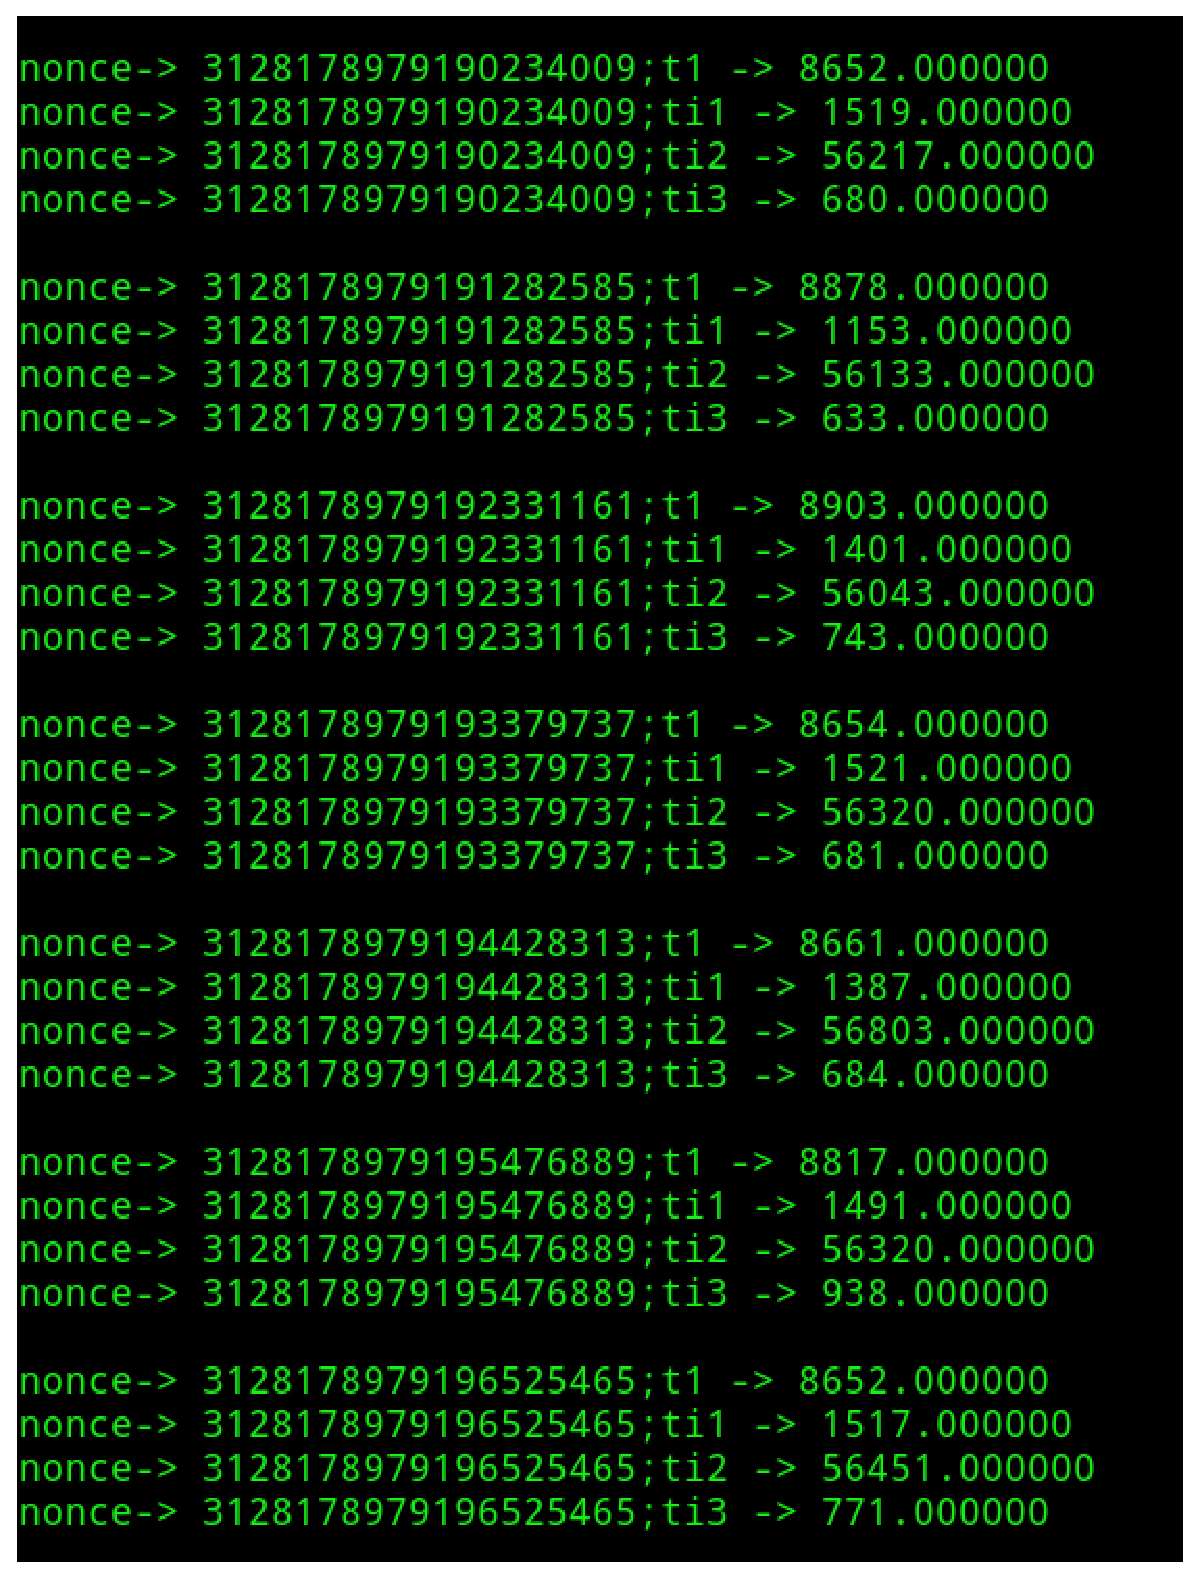
\includegraphics[width=0.8\textwidth]{ts_compute_hash.eps}
    \caption{Profiling $compute\_hash()$ by adding timestamps.}
    \label{fig:ts_compute_hash}
\end{figure}

The unit of values is the time of the GPU clock. The result indicates that the second inner iteration ti2 takes most of the time. However, it is uncertain that if different single outer iterations make inner iterations take different time. Further research is needed, which is the next week's plan.

It is noted that the implementation uses the most up-to-date CUDA APIs, like $\_\_shfl()$ and $\_\_shfl\_sync()$. Further research is needed to figure out these APIs.

\section{Miscellaneous}

\begin{itemize}
\item I decided to use Eclipse CDT to conduct experiments, which I found very convenient.
\item I have learned basic CUDA programming by official documentations and examples. Currently I have basic understanding on the Ethminer code.
\end{itemize}
%
% This section is used to list the following week's plan
% Use the \item construct to list each item.  Try to keep the
% Descriptions for each down to one or two sentences
%
\section{Next Week's Plan}
\begin{enumerate}
\item Further profile the Ethash algorithm
\item Import the Ethminer to \texttt{Nvidia Visual Profiler} and get a better profiling result
\item Produce the Stack Graph if possible
\end{enumerate}

No reference this week because the work in this week is about profiling the source code, which is fairly an engineering problem.

%\bibliographystyle{plain}
%\bibliography{references.bib}

\end{document}
